\subsection{Nuttx}
Nuttx ist ein RTOS (\acrlong{rtos}), welches auf 8 bis 32 Bit Architekturen läuft. Nuttx verwendet POSIX, damit das Operating System portierbar ist. Es ist open source, dadurch also hoch flexibel und anpassbar an die Bedürfnisse. Das Betriebssystem wird oft für kleine Embedded Systeme verwendet.
\\
Pixhawk verwendet Nuttx als Grundelement für ihre gesamte Struktur. Auf dem OS können dann mehrere Threads, sogenannte Apps, laufen. Diese verwenden das Preemtive Prinzip, also nicht kooperativ. Der Scheduler kümmert sich grösstenteils um die Einhaltung der Echtzeitkriterien.
\\
Der Cortex M4F besitzt nur 1 Kern, dadurch kann jeweils nur ein Thread laufen. Durch das Task switching können jedoch alle Tasks ihre Berechnungen durchführen. Der Scheduler, auch als Idel Task bekannt, gibt jedem Thread ein Zeitfenster, welches voll ausgenützt werden kann. Falls ein Task nicht das komplette Zeitfenster belegt, soll dieser die Ressourcen freigeben für andere Apps. Falls kein Thread Rechenzeit benötigt, wartet der Scheduler in einer Sleep ähnlichen Funktion. Im Hintergrund läuft dann der Garbage Collector und verwaltet die Speicherblöcke.\\
\\
Über eine UART (\acrlong{uart}) Schnittstelle kann man auf die nsh (\acrlong{nsh}) zugreiffen. Dies ermöglicht die Überwachung und Ausführung des Systems wie bei einem Terminal. Mit dem Befehlt top kann der Taskmanager angezeigt werden. Wie man aus der Abbildung \ref{fig:top} entnehmen kann, ist der Idel Task mit einer CPU Auslastung von 76\% stark vertreten. Die anderen Apps wie z.B. gps, px4io, sdlog2 laufen alle auch auf dem System.

\begin{figure}[ht]
  \begin{center}
  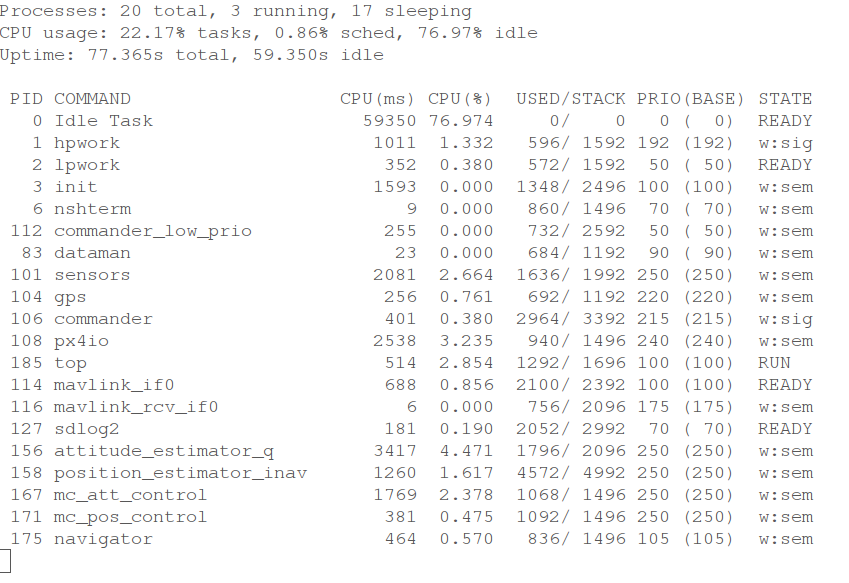
\includegraphics[scale=0.5]{pic/20_pixhawk/top2.png}
  \caption{Befehl top}
  \label{fig:top}
  \end{center}
\end{figure}

\clearpage